\subsection{Pagrindinės sistemos veikimo politikos}

Saityno peržvalgos roboto sistemų veikimo specifiką sudaro 4 pagrindinių naudojamų strategijų kombinacija. Kiekviena šių politikų yra atskira išsamiai aprašoma mokslinė saityno peržvalgos problema, reikalaujanti nuodugnios analizės, todėl šiuose punktuose šios politikos apžvelgiamos bendrais bruožais.

\subsubsection{Pasirinkimo politika}

Ši politika apibrėžia žvalgytinų puslapių prioritizavimo tvarką. Vienas didžiausių žiniatinklio žvalgymo iššūkių -- milžiniškas Interneto svetainių skaičius, kurio eksponentinis augimas išlieka iki šių dienų. Net patys efektyviausi saityno žvalgymo robotai neturi pakankamai resursų, jog galėtų padengti visas svetaines, todėl atsiranda efektyvaus prioritizavimo klausimas \cite{EffectiveWebCrawling}. Reikalinga efektyvi funkcija, kuri galėtų įvertinti žvalgytino puslapio kokybę dar prieš jį atsisiunčiant. Puslapio kokybę galima suprasti kaip kiekvieną iš šių faktorių:

\begin{itemize}
    \item Nuorodų, rodančių į puslapį, skaičius
    \item Puslapio semantinės temos atitikimas paieškos užklausai
    \item Puslapio semantikos atitikimas nuorodos tekstui
\end{itemize}

\subsubsubsection{Paieška į plotį}

Viena iš paprasčiausių žvalgymo politikų -- paieškos į plotį algoritmas, kurio principas pavaizduotas \ref{fig:bfs} paveikslėlyje. Atlikti eksperimentiniai žvalgymo tyrimai (aplankyta virš 300 mln. svetainių) parodė, jog paieškos į plotį strategija puikiai veikia surenkant aukštos kokybės puslapius žvalgymo pirmuose etapuose \cite{EffectiveWebCrawling}. Ši išvada grįsta nuomone, kad aukštesnės kokybės puslapiai turi daugiau nuorodų, vedančių į juos, todėl atrandami anskčiau \cite{EffectiveWebCrawling}.

\begin{figure}[htp!]
\centering
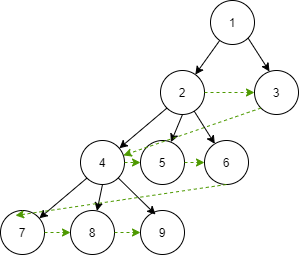
\includegraphics[scale=0.7]{img/BFS.png}
\caption{Paieškos į plotį grafas}
\label{fig:bfs}
\end{figure}

\subsubsubsection{PageRank algoritmo metrika}

Kitas būdas atlikti efektyvesnį žvalgymą -- kiekvienam lanktytinam puslapiui apskaičiuoti kokybės metriką ir lankyti aukštos metrikos vertės puslapius anskčiau. Viena iš tokių metrikų -- „Google“ patentuotas ir šios kompanijos pirmasis svetainių kokybės vertinimo algoritmas „PageRank“.

\begin{figure}[htp!]
\centering
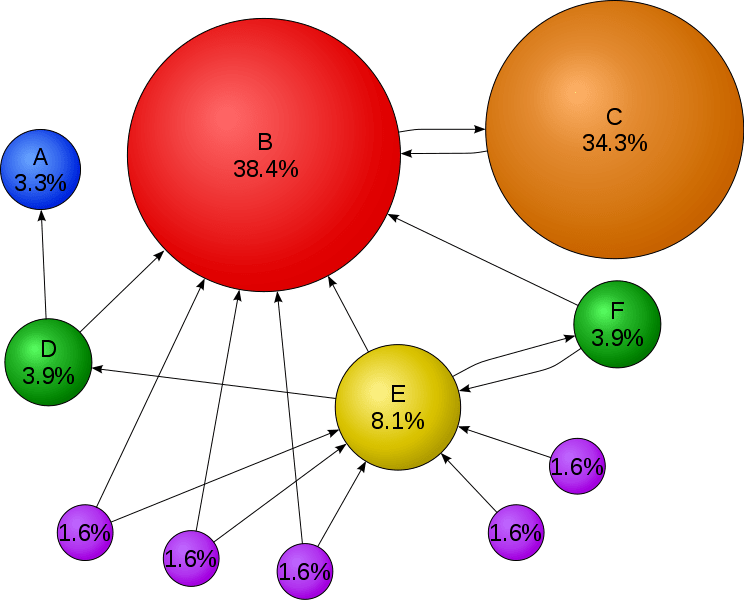
\includegraphics[scale=0.4]{img/pagerank.png}
\caption{„PageRank“ algoritmo principas \cite{PageRank}}
\label{fig:pagerank}
\end{figure}

Kaip galima pastebėti iš \ref{fig:pagerank} grafo, „PageRank“ algoritmas vertina nuorodų skaičių, kurios rodo į tam tikrą puslapį ir tų nuorodų puslapių kokybę. Matoma, jog B viršūnė turi aukštą autoritetą, nes į ją rodo daug mažų viršūnių, o C viršūnė -- nes į ją rodo viena aukšto autoriteto viršūnė.

\subsubsection{Etiško žvalgymo politika}

Saityno žvalgymo robotai veikia naudodami daug lygiagrečių žvalgymo procesų, kurie sugeneruoja didelius kiekius tinklo I/O srauto. Žvalgant konkretų žiniatinklio serverį, svarbu užtikrinti, jog priskirtas žvalgymo procesas nesutrikdytų sklandaus šio serverio darbo, t.y. nesukeltų netyčinės DoS\footnote{DoS - Denial of Service Attack} atakos \cite{EffectiveWebCrawling}. 

\subsubsubsection{REP protokolas}

Kaip dalinė etiško saityno žvalgymo užtikrinimo priemonė, buvo sukurtas \textit{Robots Exclusion Protocol} taisyklių rinkinys, kuriuo svetainių administratoriai gali nurodyti, kurias svetainės dalis jie leidžia robotams pasiekti, taip pat, koks galimas minimalus žvalgymo užklausų laiko intervalas. Pavyzdinis robots.txt failo turinys matomas \ref{fig:rep-example} paveikslėlyje.

\begin{figure}[htp!]
\centering
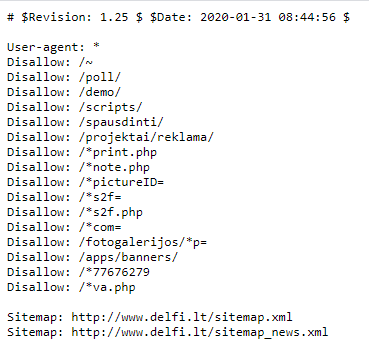
\includegraphics[scale=0.8]{img/rep_protocol.png}
\caption{delfi.lt robots.txt pavyzdys}
\label{fig:rep-example}
\end{figure}

\textit{User-agent} direktyva apibrėžia robotų pavadinimus, kuriems taikomas taisyklių rinkinys. Kiekvienas etiškas žvalgymo robotas kreipdamasis į žiniatinklio serverį identifikuoja save naudodamas šią HTTP antraštės reikšmę. Pavyzdžiui, „Googlebot“ sistema naudoja tokią šios HTTP antraštės reikšmę:
\begin{verbatim}
Mozilla/5.0 AppleWebKit/537.36 (KHTML, like Gecko; compatible; Googlebot/2.1; 
+http://www.google.com/bot.html) Chrome/W.X.Y.Z‡ Safari/537.36
\end{verbatim}
\textit{Disallow} direktyva nurodo, koks dokumentas ar byla negali būti pasiekiama tam tikram robotui. Taip pat gali būti naudojamas „*“ simbolis (\textit{angl. -- wildcard symbol}), nurodantis, jog taisyklių rinkinys turi būti taikomas bet kokiai reikšmei \cite{RobotsExclusionProtocol}.

Į oficialių standartą neįtraukta, bet dažnai sutinkama \textit{Crawl-delay} direktyva, kurią kiekvienas žvalgymo robotas gali interpretuoti skirtingai, dažniausiai tai būna laiko tarpas tarp skirtingų HTTP užklausų į serverį.

Akcentuotina, kad šis protokolas negarantuoja, jog robotas nežvalgys uždraustų direktorijų ar resursų, nes žiniatinklyje yra daugybė neetiškų žvalgymo sistemų, siekiančių blogų tikslų.

\subsubsubsection{Svetainės žvalgymo intervalai}

Ši roboto sistemos charakteristika yra svarbiausia etiško žvalgymo politikoje. Turi būti išlaikytas balansas tarp žvalgymo mandagumo (neapkraunamas žiniatinklio serveris) ir peržvalgos efektyvumo, nes didelės svetainės, turinčios šimtus tūkstančių puslapių, turi būti žvalgomos itin greitai \cite{EffectiveWebCrawling}.

\subsubsection{Pakartotinio apsilankymo politika}

Inkrementinio tipo žvalgymo robotai turi užtikrinti, jog sistemos puslapių indekso repozitorijoje turimos lokalios puslapių kopijos yra kiek galima naujesnės ir atitinkančios originalų resursą esamu laiku. \cite{EffectiveWebCrawling}

Šiam tikslui yra apibrėžtos dvi pagrindinės funkcijos, sutinkamos literatūroje, kurios kartu nusako puslapio pokyčio neaptikimo kainą.

\subsubsubsection{Šviežumo funkcija}

Ši funkcija nusako, ar lokali kopija atitinka originalų resursą duotuoju laiko momentu ir gali būti apibrėžiama taip:

\[F\: p(t) = \left\{\begin{matrix} 1, & p & puslapis & atitinka & laiko & momentu & t\\ 0 & kitu & atveju \end{matrix}\right.\]

\subsubsubsection{Amžiaus funkcija}

Ši funkcija nusako, kokio senumo turima lokali puslapio p kopija:

\[A\: p(t) = \left\{\begin{matrix} 0, & p & puslapis & nepakeistas & laiko & momentu & t\\ t & kitu & atveju \end{matrix}\right.\]

\textit{t} reikšmė šiuo atveju nusako puslapio modifikavimo laiką.

\subsubsubsection{Pakartotinio apsilankymo strategijos}

Pagal \cite{EffectiveWebCrawling} dažniausiai sutinkamos 2 pakaertotinio žvalgymo strategijos:

\begin{enumerate}
    \item Vieningoji strategija -- visi puslapiai pakartotiniai žvalgomi kas tą patį laiko intervalą
    \item Proporcinė strategija -- dažniau kintantys puslapiai žvalgomi dažniau
    \item Svarbos strategija -- svarbesni puslapiai (taikomos metrikos įvertinti, pvz.: „PageRank“) žvalgomi dažniau
\end{enumerate}

Ištirta, jog vieningoji strategija plačiajame žvalgyme efektyvesnė už proporcinę \cite{EffectiveWebCrawling}.